\documentclass[a4paper, 12pt]{article}
\usepackage[utf8]{inputenc}
\usepackage[T2A]{fontenc}
\usepackage{amsmath,amssymb,amsthm}
\usepackage[a4paper,hmargin=2.5cm,vmargin=2.5cm]{geometry}
\usepackage[english]{babel}
% \usepackage{graphics}
\usepackage{float}
\usepackage{graphicx}
\usepackage{xcolor}
\usepackage{hyperref}

\DeclareMathOperator{\argmax}{argmax}
\DeclareMathOperator{\Image}{Im}

\graphicspath{{./images/}}

\theoremstyle{definition}
\newtheorem{definition}{Definition}[section]


\theoremstyle{definition}
\newtheorem{example}{Example}[section]

\newtheorem{theorem}{Theorem}

\theoremstyle{remark}
\newtheorem*{remark}{Remark}

\newcommand\myworries[1]{\textcolor{red}{#1}}


\begin{document}

\renewcommand{\labelenumii}{\arabic{enumi}.\arabic{enumii}}
\renewcommand{\labelenumiii}{\arabic{enumi}.\arabic{enumii}.\arabic{enumiii}}
\renewcommand{\labelenumiv}{\arabic{enumi}.\arabic{enumii}.\arabic{enumiii}.\arabic{enumiv}}

%%
%% Title page
%%
\begin{center}
{\scshape National Research University\\
Higher School of Economics\\[1ex]
Faculty of Mathematics\par}

\par\vfill

\textbf{\large Project Proposal}

\vspace{1.5cm}

{\Large\bfseries
Clustering of Multidimensional Random Variables to Improve HMM Sequence Alignment Accuracy \\

Кластеризация многомерной случайно величины для поднятия точности выравнивания строк.
\par}

\vspace{1.5cm}

\par\vfill
\noindent\hspace{0.52\textwidth}\parbox[t]{0.48\textwidth}{%
Student: Denis Grachev, БМТ181\\[2ex]
}

\par\vfill
\noindent\hspace{0.52\textwidth}\parbox[t]{0.48\textwidth}{%
Scientific advisor:\\[3pt]
PhD candidate, \\ 
Timofey Prodanov\\[2ex]
}

\par\vfill\vfill
Moscow 2022
\end{center}
\thispagestyle{empty}
\pagebreak

%%
%% ===========================================================================
%%

\tableofcontents
\newpage

\section{Abstract}

Whole-genome sequencing is a complex and important task of bioinformatics. 
Different technologies can generate data of different nature. 
Most popular technologies, such as Illumina, 
have low error rate, but give limited information about genome.
Newer technologies, for example Pacific Biosciences and Oxford Nanopore, 
can give more details about genome, but have higher error rate. 
Combination of these methods can help improve accuracy of genome sequencing. 
During this work a new method of string clustering was developed, 
to identify different data profiles and new functionality to existing tools were added,
to work with multiple datasets. 

\section{Introduction}
Bioinformatics is an interdisciplinary science that aims 
to develop methods and software tools 
for understanding biological data. 
The most useful biological analysis is related to DNA (genome) exploration. 
One of the ways to represent genome is as a set of strings over the alphabet $\{ A, C, G, T \}$, 
each corresponding to a chromosome.
Most species are diploid, so every chromosome is paired, one copy from each parent.  
Modern technologies of reading human genome (genome sequencing), 
such as Illumina \cite{goodwin2016coming},  
do not allow to read it as one 
continuous string, but a number of random substrings 
that are called reads. 
In most species unrelated individuals have highly similar genome sequences 
(99.9\% among humans \cite{NationalHumanGenome})  
As within one biological species genomes coincide almost completely, 
it is convenient to determine one reference genome for one species 
and identify for every individual it's deviations from the reference.
Most common deviations are single nucleotide substitutions, which are called SNVs.
A number of problems appears for example:
\begin{itemize}
    \item \textbf{Genome assembly} is process of  
    deciphering genome using reads obtained from it.
    
    \item \textbf{Sequence alignment} is process of 
    arranging sequences to spot similarities between them. 
    
    \item \textbf{Variant calling} is process of identifying 
    SNVs of an individual based on reads aligned on the reference genome.
\end{itemize}
Solving this problems are complicated by errors in genome sequencing. 
The most commonly used technologies, Illumina \cite{goodwin2016coming}, 
allow to sequence reads of length 200-500 bp.
Sequencing human genome using such short length reads 
has many limitations. 
First, due to diploidy of humans, it is important to obtain
long-range relation between SNVs on each homologous chromosome. This might be difficult 
with short-reads provided by Illumina \cite{goodwin2016coming}. 
Second, $~3.6\%$ \cite{edge_longshot_2019} of 
human genome consists of long highly repetitive 
duplicated regions. Calling SNVs in such regions using short-read sequencing technologies 
is increasingly difficult, which lowers accuracy of SNVs. 
Third-generation single-molecule sequencing (SMS) technologies,
such as Oxford Nanopore Technologies (ONT) \cite{jain2016oxford} and 
Pacific Bioscience (PacBio) \cite{rhoads2015pacbio} allow to   
generate longer reads of length 10-30 kb, however they exhibit higher error rates.
These technologies might help overcome limitations that short-reads have. 
Variant calling tools that were developed 
for short-reads, such as GATK HaplotyperCaller \cite{mckenna2010genome} and 
FreeBayes \cite{garrison2012haplotype} do not show high accuracy when applied 
to long-reads sequencing, due to significant difference 
in error rates and type of errors between these two types of reads. 
Also these tools process data in short windows 
of a few hundred bases lengths and are not designed to aggregate  
haplotype information present in long-reads, 
which might be crucial for distinguishing true deviations 
from errors.  \\
A number of new methods of variant calling were developed 
to work with long-reads, such as Deepvariant \cite{poplin2018universal}
and Longshot \cite{edge_longshot_2019} that use deep learning 
and pair-Hidden Markov model algorithms to effectively work with such data. 
Accuracy of these methods can be improved by efficiently using information 
obtained with different technologies.  
Spades \cite{bankevich2012spades} genome assembly tool is an example of effectiveness 
of sequence data aggregation.

Longshot variant calling tool is able to process standard long-read sequencing datasets 
as well as HiFi (CCS) \cite{wenger2019accurate} data, but it is unable to usefully combine 
multiple datasets at the same time. 
By effectively aggregating data from different sequencing sources 
we can improve Longshot \cite{edge_longshot_2019} sensitivity and accuracy.
Previous research show that sequencing reads of 
different profiles and clustering them 
by their profiles can improve variant calling accuracy.
% If true add reference

In this paper we are extending the functionality of 
Longshot tool to work effectively with multiple datasets. 
For that we developed a clustering algorithm for 
read profiles and implemented such feature into Longshot. 

\section{Preliminaries}
\subsection{Strings}

\begin{definition}
    String is a sequence of letters of finite size. \\
    String of length $l$ over alphabet $A = \{ 1 \ldots m \}$ is a map $s: \{ 1 \ldots l\} \rightarrow A$.
    Usually elements of $A$ are denoted as characters for convenience.
\end{definition}

\begin{definition}
    Alignment of strings is a way of representing them to spot similarities. \\
    Alignment of strings $s_1$ and $s_2$ of lengths $l_1$ and $l_2$ respectively, 
    over alphabet $A$ is a pair of strings $\hat{s}_1$ and $\hat{s}_2$ 
    of length $l$ over alphabet $A \sqcup \{ '-' \}$, 
    such that there exists increasing functions $f_i: \{1 \ldots l_i \} \rightarrow \{ 1 \ldots l\}, i \in \{1, 2\}$ 
    such that $\hat{s}_i \circ f_i = s_i$ and $\Image (f_i) = \hat{s}_i^{-1}(A)$. \\

    Letter $'-'$ represents gap in a string. 
    String $\hat{s}_i$ represents string $s_i$ with inserted letter $'-'$, 
    that was not present in alphabet $A$, into some places, 
    and function $f_i$ maps indexes of letters in $s_i$ to corresponding indexes in $\hat{s}_i$.
\end{definition}

\begin{example}
    Alignment of strings $s_1 = CABCAABA$ and $s_2 = ABADBBAD$ 
    over alphabet $\{ A, B, C, D\}$.

    \begin{center}
        Initial strings. \\
        \begin{tabular}{|| c | c c c c c c c c ||}
         $s_1$ & C & A & B & C & A & A & B & A \\ 
         $s_2$ & A & B & A & D & B & B & A &   \\    
        \end{tabular}

        \hfill \break 

        Aligned strings. \\
        \begin{tabular}{|| c | c c c c c c c c c ||}
            $\hat{s}_1$ & C & A & B & C & - & A & A & B & A \\ 
            $\hat{s}_2$ & - & A & B & - & A & D & B & B & A   
        \end{tabular}

    \end{center}
\end{example}


% \begin{theorem}
%     If $G$ is symmetric and 
%     $
%     g_{ij} =
%         \left\{\begin{array}{cc}
%         0, & i = j\\
%         >0, & 
%         \end{array}\right.
%     $ and $p > 0$, then we can define metric for strings over alphabet $A$ as 
%     $$ d(s_1, s_2) = \min \{S(\hat{s}_1, \hat{s}_2)\}$$ 
% \end{theorem}

% \begin{proof}
    
% \end{proof}

\begin{definition}
    Define score function for an alignment $S(\hat{s}_1, \hat{s}_2)$. 
    The \emph{better} alignment the more score it gets. 
    Different score functions will be introduced later.
\end{definition}

\begin{definition}
    We are interested in the alignment with the highest possible score. 
    So we define score between two strings as 
    $$ S(s_1, s_2) = \max_{\hat{s}_1, \hat{s}_2} S(\hat{s}_1, \hat{s}_2 )$$ 
\end{definition}

\begin{definition}
    Substring is continuous piece of a given string.\\
    For a string $s$ of length $l$, sub-string $s_s$ 
    is a string of length $l_s$, such that there exists a function
    $f: \{ 1 \ldots l_s \} \rightarrow \{ 1 \ldots l\}$
    such that
    $$ f(i) = i + d $$
    $$s \circ f = s_s.$$
\end{definition}

\begin{definition}
    We want to find similarities between reference string and reads. 
    For this we define local alignment and score for a string and a substring. \\  
    For a string $s_1$ and $s_2$ of lengths $l_1, l_2$ correspondingly, define string-sub-string score as 
    $$ S_s (s_1, s_2) = \max \{ S(s_s, s_2) \:|\: s_s \text{ is a sub-string of } s_1 \}$$
    and corresponding alignment $\hat{s}_1, \hat{s}_2$.
\end{definition}

\begin{definition}
    For a string $s$ of length $l$ and set of strings $R = \{ s_1 \ldots s_n \}$ 
    of lengths $\{ l_1 \ldots l_n \}$ correspondingly, 
    multiple alignment is tuple $\hat{s}, \hat{s}_1 \ldots \hat{s}_n$, 
    of strings of length $l$ over alphabet $A \sqcup \{ '-' \}$, such that $\sum_{i = 1}^n S(\hat{s}, \hat{s}_i)$ is maximal.
\end{definition}

\begin{definition}
    Set of reads $R$ for string $s$ of length $l$ and rate $r$ is 
    $$ R = \{ s_s \:|\: \text{length of } s_s > l, S_s(s, s_s) < r \}$$
\end{definition}

\subsection{Task}
Given reference string $s_r$ and reads $R$ for an unknown target string $s_t$, 
we know that $S(s_r, s_t) < D$ and want to find $s_t$. \\

Plan:
\begin{enumerate}
    \item Make multiple alignment of $R$ over $s_r$.
    \item Estimate most likely difference between $s_r$ and $s_t$.
\end{enumerate}

\begin{figure}[H]
    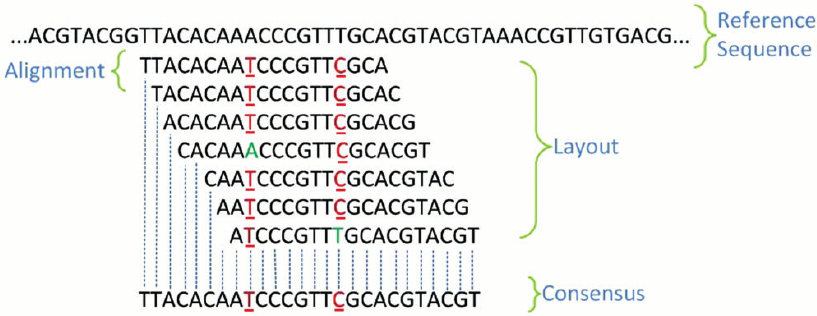
\includegraphics[scale=0.5]{aligned_reads.png}
    \centering
    \caption{Example of reference string, target string and reads.}
\end{figure}

\subsection{Additive scoring functions}

One of the ways to score an alignment is to add award for matches and 
subtract penalty for mismatches and gaps. 

\begin{definition}    
    For a given matrix $G \in \mathbb{R}^{|A \sqcup \{ '-' \} | \times |A \sqcup \{ '-' \}|}$ and $p \in \mathbb{R}$ 
    score of alignment $\hat{s}_1, \hat{s}_2$ is 
    $$ S(\hat{s}_1, \hat{s}_2) = \sum_{i = 1}^l G_{\hat{s}_1(i), \hat{s}_2(i)}. $$
    %     \text{ where } 
    %     \delta_{i}=
    %         \left\{\begin{array}{cc}
    %         g_{\hat{s}_1(i) \hat{s}_2(i)},& \hat{s}_1(i) \neq - \text{ and } \hat{s}_2(i) \neq -\\
    %         p, & 
    %         \end{array}\right. 
    % $$
    Matrix $G$ stores predefined penalties for mismatches and 
    gaps and encouragement for matches. \\
    Sometimes fines penalty for first gap is higher than prolonging a continuous gap, 
    because one continuous gap is more likely to appear than several small gaps. \\
    Best alignment for such score function can be found using Needleman-Wunsch algorithm.

\end{definition}

\subsection{Pair Hidden Markov Model}
Each step of pairwise alignment can be assigned to one of 
the three states $\{ M, X, Y\}$, where $M$ is a match, 
$X$ is a gap in $s_1$, $Y$ is a gap in $s_2$. 
Given transition probabilities each alignment can be assigned a probability.
The most likely alignment can be found using Viterbi algorithm.
% \myworries{Add about begin and end states?}

\subsection{Clustering}
\begin{definition}
    Clustering algorithm aims to group points together into predefined number of sets. \\
    Clustering algorithm is a map 
    $$\text{cluster} (X, m) \rightarrow C$$
    $$X = \{x_i \:|\: x_i \in \mathbb{R}^d, i \in \left( 1 \ldots n \right) \}, \; m \in \mathbb{N}$$
    $$C = \{ c_i \:|\: c_i \in \left( 1 \ldots m \right), i \in \left( 1 \ldots n \right)\}$$
    where $m$ is number of clusters and $n$ is number of points. 
\end{definition}

\begin{figure}[H]
    
\includegraphics{example_clustering}
    \centering
    \caption{Example of clustering for $d=2$, $m=2$, color represents class.}
\end{figure}

\subsection{Stepwise iterative maximum likelihood algorithm (SIML)}
To distinguish different read profiles a new method of clustering was developed.
\subsection{Likelihood}

Assume that the data consists of different multidimensional normal distributions. \\
Let's denote data as  
$$X = \{x_i \:|\: x_i \in \mathbb{R}^d, i \in \left( 1 \ldots n \right) \}, m \in \mathbb{N}$$
where $m$ is number of clusters and $n$ number of points. 
Assume that we have some clustering $C$, we will try to increase it's likelihood. \\
Denote ith cluster as $\omega_i$ and it's estimated parameters as $\theta_i$
$$ \Theta = \{ \theta_i \:|\: i \in (1 \ldots m)\}.$$
Then probability of $x$ in ith cluster
$$ p(x \:|\: \Theta) = p(x \:|\: \omega_i, \theta_i) P(\omega_i).$$
Denote clusters as $ \chi_1 \ldots \chi_l \subset X $, 
than logarithm of probability for all points in cluster i is 
\begin{align*}
    L_i &= \sum_{x \in \chi_i} \log(p(x \:|\: \omega_i, \theta_i)P(\omega_i)) \\
        &=  \log \left( 
        \frac{ \exp \left( \frac{-1}{2} (x - \mu_i)^T \Sigma_i^{-1} (x - \mu_i) \right) }
        {(2 \pi)^{d/2} |\Sigma_i| ^ {1/2}}
        \right) + n_i \log(P(\omega_i)) \\
        &= -\frac{1}{2} n_i d - \frac{n_i d}{2} \log(2 \pi) - \frac{n_i}{2} \log |\Sigma_i| + n_i \log \frac{n_i}{n}.
\end{align*} 
Where $\mu_i$ is mean value and $\Sigma_i$ - covariation of ith cluster.
Overall likelihood is 
$$ L = \sum_{i = 1}^l L_i.$$
Move $\hat{x}$ from $\chi_i$ to $\chi_j$, then

\begin{align*}
    \Delta L_i = &-\frac{1}{2} \log |\Sigma_i| + \frac{n_i - 1}{2} 
        \log \left(1 - \frac{(\hat{x} - \mu_i)^T \Sigma_i^{-1}(\hat{x} - \mu)}{n_i - 1} \right) + \\
         &+ \log \frac{n_i}{n} - (n_i - 1)(\frac{d}{2} + 1) \log \frac{n_i - 1}{n_i}
\end{align*}

\begin{align*}
    \Delta L_j = &-\frac{1}{2} \log |\Sigma_j| - \frac{n_j + 1}{2} 
        \log \left(1 + \frac{(\hat{x} - \mu_j) \Sigma_j^{-1} (\hat{x} - \mu_j)}{n_j + 1}\right) + \\
         &+ \log \frac{n_j}{n} + (n_j + 1)(\frac{d}{2} + 1) \log \frac{n_j + 1}{n_j}.
\end{align*}

\begin{align*}
    \Delta L &= \Delta L_i + \Delta L_j
\end{align*}

\subsection{Algorithm}
Main idea
\begin{enumerate}
    \item Initialize clusters (randomly or using another algorithm)
    \item Iterate over all points
    \begin{enumerate}
        \item Move point to a cluster, such that overall likelihood increases the most. (With most $\Delta L_j$)
        \item Update clusters and their parameters.
    \end{enumerate}
    \item Repeat step 2 while it makes changes.
\end{enumerate}
Advantages
\begin{itemize}
    \item After every step overall likelihood increases.
    \item This implies that the cycle will end.
\end{itemize}
Problems
\begin{itemize}
    \item Updateting parameters after every step is very slow.
\end{itemize}
Transition of one point does not change estimated parameters significantly, 
so to reduce iteration complexity, we will update parameters once in $k$ points. 
Also to avoid possible loops we will iterate over points in different orders. \\
Final algorithm:
\begin{enumerate}
    \item Initialize clusters and estimate their parameters
    \item Decide $X$ into $p$ random disjoint groups $g_1 \ldots g_p$.
    \item Loop c from $1$ to $p$.
    \begin{enumerate}
        \item Loop $x$ over $g_c$.
        \begin{enumerate}
            \item Let $x$ currently be in cluster $i$.
            \item If $n_i <= 1$, then pass to next point.
            \item Calculate $\delta_{j}=
                \left\{\begin{array}{cc}
                \Delta L_{j}, & j \neq i \\
                \Delta L_{i}, & j=i
                \end{array}\right. $
            \item Transfer $x$ to $\argmax (\delta_j)$ cluster.
        \end{enumerate} 
        \item Update parameters.
        \item If overall likelihood is not increased, revert changes.
    \end{enumerate}
    \item If any changes were made, repeat step 2.
\end{enumerate}

\begin{theorem}
    Proposed algorithm is finite.    
\end{theorem}
\begin{proof}
    As there are $m^n$ different clusterings, we can order them by their likelihood.
    After every processed group $g_c$ total likelihood is increased or clustering is not changed, 
    hence we cannot be looped, because we can not increase likelihood infinitely many times, 
    and when no changes were made the algorithm stops.  
\end{proof}


\section{Main results}
\subsection{Clustering}
The algorithm was tested on data generated by simlord \cite{stocker2016simlord} 
with different generating parameters. For every read 
\begin{itemize}
    \item length,
    \item number of matches,
    \item number of mismatches,
    \item number of insertions (gaps in reference),
    \item number of deletions (gaps in read),
    \item number of all transitions from states match, mismatch, insertion, deletions,
    \item length of left soft-clipping (continuous region of mismatches before first match, insertion or deletion),
    \item length of right soft-clipping (continuous region of mismatches after last match, insertion or deletion). 
\end{itemize}
were calculated. \\
For clustering 
\begin{itemize}
    \item number of all transitions from states match, mismatch, insertion, deletions,
    \item length of left soft-clipping,
    \item length of right soft-clipping      
\end{itemize}
were used. \\
To make read's profile independent from it's length, 
all transitions were divided by length of the read.
Also all features were normalized by their standard deviations, 
to equal their contribution when calculate distance between points.
After that PCA method \cite{abdi2010principal} was applied to the data, 
to reduce linear dependencies and extract important information.
To make comparison with existing clustering algorithms,
preproccessed data was clustered by 3 groups using  
Kmeans \cite{sklearn_api}, Gaussian mixture \cite{sklearn_api} and SIML clustering algorithms.
Axes represent two main PCA components, color represent cluster.
\begin{figure}[H]
    \minipage{0.32\textwidth}
      \includegraphics[scale=0.4]{kmeans_generated_3}
      \caption{K-Means}
    \endminipage\hfill
    \minipage{0.32\textwidth}
      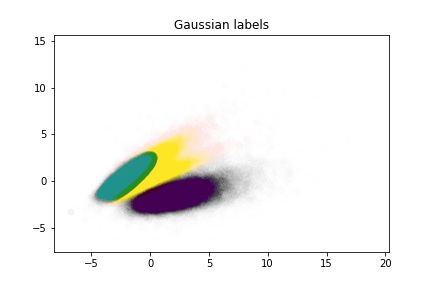
\includegraphics[scale=0.4]{gaussian_generated_3}
      \caption{GaussianMixture}
    \endminipage\hfill
    \minipage{0.32\textwidth}
    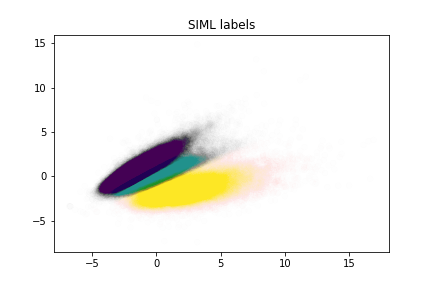
\includegraphics[scale=0.4]{siml_generated_3}
    \caption{SIML}
    \endminipage
\end{figure}
For SIML we can see how likelihood of clustering changed over iterations.

\begin{figure}[H]
    \begin{center}
    \minipage{0.49\textwidth}
      \includegraphics[scale=0.49]{siml_likelihood_3.png}
      \caption{Likelihood history over iterations.}
    \endminipage
    \end{center}
\end{figure}
More precise testing is yet to be completed. 
Algorithm was \href{https://github.com/grach0v/my_SIML}{implemented} using python. 

\subsection{Longshot}
\href{https://github.com/grach0v/longshot}{Fork} of Longshot \cite{edge_longshot_2019} with features of clustering and processing multiple 
datasets is in development.  

\newpage

\bibliography{refs} 
\bibliographystyle{ieeetr}

% \newpage
% \begin{thebibliography}{00}
%     % TODO change reference
    
% \end{thebibliography}

\end{document}

